\documentclass{IEEEcsmag}

\usepackage[colorlinks,urlcolor=blue,linkcolor=blue,citecolor=blue]{hyperref}
\expandafter\def\expandafter\UrlBreaks\expandafter{\UrlBreaks\do\/\do\*\do\-\do\~\do\'\do\"\do\-}
\usepackage{upmath,color}

\usepackage[spanish]{babel}
%\usepackage[latin1]{inputenc}
\usepackage[utf8]{inputenc}  

\jvol{1}
\jnum{1}
\paper{1}
\jmonth{Noviembre}
\jname{ITICs letters}
\jtitle{Proyectos Integradores}
\pubyear{2023}

\newtheorem{theorem}{Theorem}
\newtheorem{lemma}{Lemma}



\setcounter{secnumdepth}{0}

\begin{document}

\sptitle{Proyecto Integrador de Primer Semestre}

\title{Software de resolución de problemas de Ingeniería }

%primer autor
\author{\IEEEauthorblockN{1\extsuperscript{er} Calva Abraham}
\IEEEauthorblockA{\textit{Estudiante de iTIC'S} \\
\textit{ITSOEH}\\
Mixquiahuala, Hgo. \\
230110637@itsoeh.edu.mx}
\and

%segundo autor
\IEEEauthorblockN{2\textsuperscript{do} Vidal Ceron Jean Paul}
\IEEEauthorblockA{\textit{Estudiante de iTCS'S} \\
\textit{ITSOEH}\\
Mixquiahuala, Hgo. \\
230110625@itsoeh.edu.mx}
\and
%tercer autor
\IEEEauthorblockN{3\textsuperscript{o} Martinez Escamilla Erick}
\IEEEauthorblockA{\textit{Estudiante de iTCS'S} \\
\textit{ITSOEH}\\
Texcatepec, Hgo. \\
230110626@itsoeh.edu.mx}
\and

%cuarto autor
\IEEEauthorblockN{4\textsuperscript{o} Barrera Rojo Roberto}
\IEEEauthorblockA{\textit{Estudiante de iTCS'S} \\
\textit{ITSOEH}\\
Mixquiahuala, Hgo. \\
230110946@itsoeh.edu.mx}
\and

%quinto autor
\IEEEauthorblockN{5\textsuperscript{o} Jacob Salas Andrea}
\IEEEauthorblockA{\textit{Estudiante de iTCS'S} \\
\textit{ITSOEH}\\
Santiago de Anaya, Hgo. \\
230110449@itsoeh.edu.mx}
\and
}

\maketitle
\clearpage
\onecolumn
\tableofcontents
\clearpage
\twocolumn

\markboth{ITSOEH/ITICS/PROYECTO INTEGRADOR PRIMER SEMESTRE}{THEME/FEATURE/DEPARTMENT}

\begin{abstract}
En este documento se presentan diversas estrategias para abordar desafíos en la electrónica, redes, seguridad y su aplicación en el campo de la ingeniería en telecomunicaciones y tecnologías de la información y comunicación para los estudiantes.
\end{abstract}

\maketitle


\chapteri{E}n el campo de la ingeniería, la resolución de problemas es esencial y requiere precisión, conocimiento y eficiencia. Este proyecto tiene como objetivo diseñar y desarrollar software especializado en la resolución de problemas de ingeniería. Cada software proporciona funciones clave para abordar problemas específicos. Se utiliza la metodología de las 6D, que incluye la descripción del problema, la definición de la solución, el diseño de la solución, el desarrollo de la solución, la depuración y las pruebas, y finalmente la documentación.

El propósito de este proyecto integrador es ofrecer herramientas que abarquen diversas áreas matemáticas relevantes en la ingeniería, con el fin de resolver problemas de manera eficiente y precisa, optimizando así el tiempo de trabajo.

\section{Ecuación de la recta}
%Solución del Ejercicio 1 por medio de la metodología 6D

\subsection{Descripción del problema}
Dados 2 puntos $A \mbox{ y } B$ con coordenadas $x_{1}, y_{1}$ y $x_{2}, y_{2}$  respectivamente. Regresar la ecuación de la recta y el ángulo interno $\alpha$ que se forma entre el eje horizontal y la recta. 
%Por ejemplo con los puntos $A(2, 1)$ y $B(-3, 2)$ la ecuación debe ser $y = -\frac{1}{5}x + \frac{7}{5}$. 

\begin {figure}[h!]
\centerline{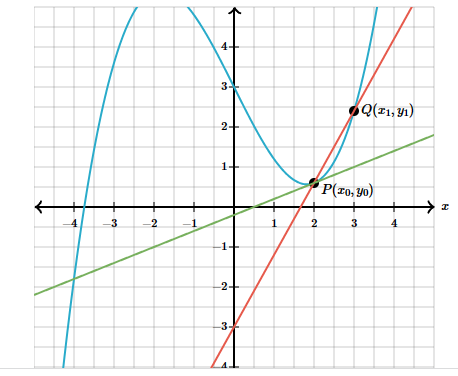
\includegraphics[width = 6cm]{Latex-imágenes/fig1 latex.png}}
\caption{Gráfica de la ecuación de la recta.}
\label{fig}
\end {figure}


\subsection{Definición del problema}
En la ecuación de la recta si dos puntos distintos $P(x_{1},y_{1})$ y $Q(x_{2},y_{2})$ se ubican en la curva $y=f(x)$ , la pendiente de la recta secante que uno los dos puntos es:

\begin{equation}
m_{sec} = \frac{y_{2} - y_{1}} {x_{2}- x_{1}} = \frac{F({x_{2}}) - {F({x_{1}})}} {x_{2}-x_{1}}
\end{equation}

Para identificar la intersección en el eje vertical se utiliza cualquiera de los 2 puntos para este caso se utilizo $P(x_{1},y_{1})$ de la siguiente forma:
\begin{equation}
    b = y_{1-} - m_{sec} * x_{1} 
\end{equation}

utilizando este método, puedes encontrar la ecuación de la recta a partir de 2 puntos dados.
y para calcular el ángulo de dicha pendiente se usa:

\begin{equation}
    \sphericalangle=\arctan(m)
\end{equation}
el algoritmo de solución implementado en el lenguaje Java empieza por la entrada de los valores $P(x_{1},y_{1})$ y $Q(x_{2},y_{2})$ solicitando sean separados por una coma.

\subsection{Diseño de la solución}
\begin {figure}[htb]
\centerline{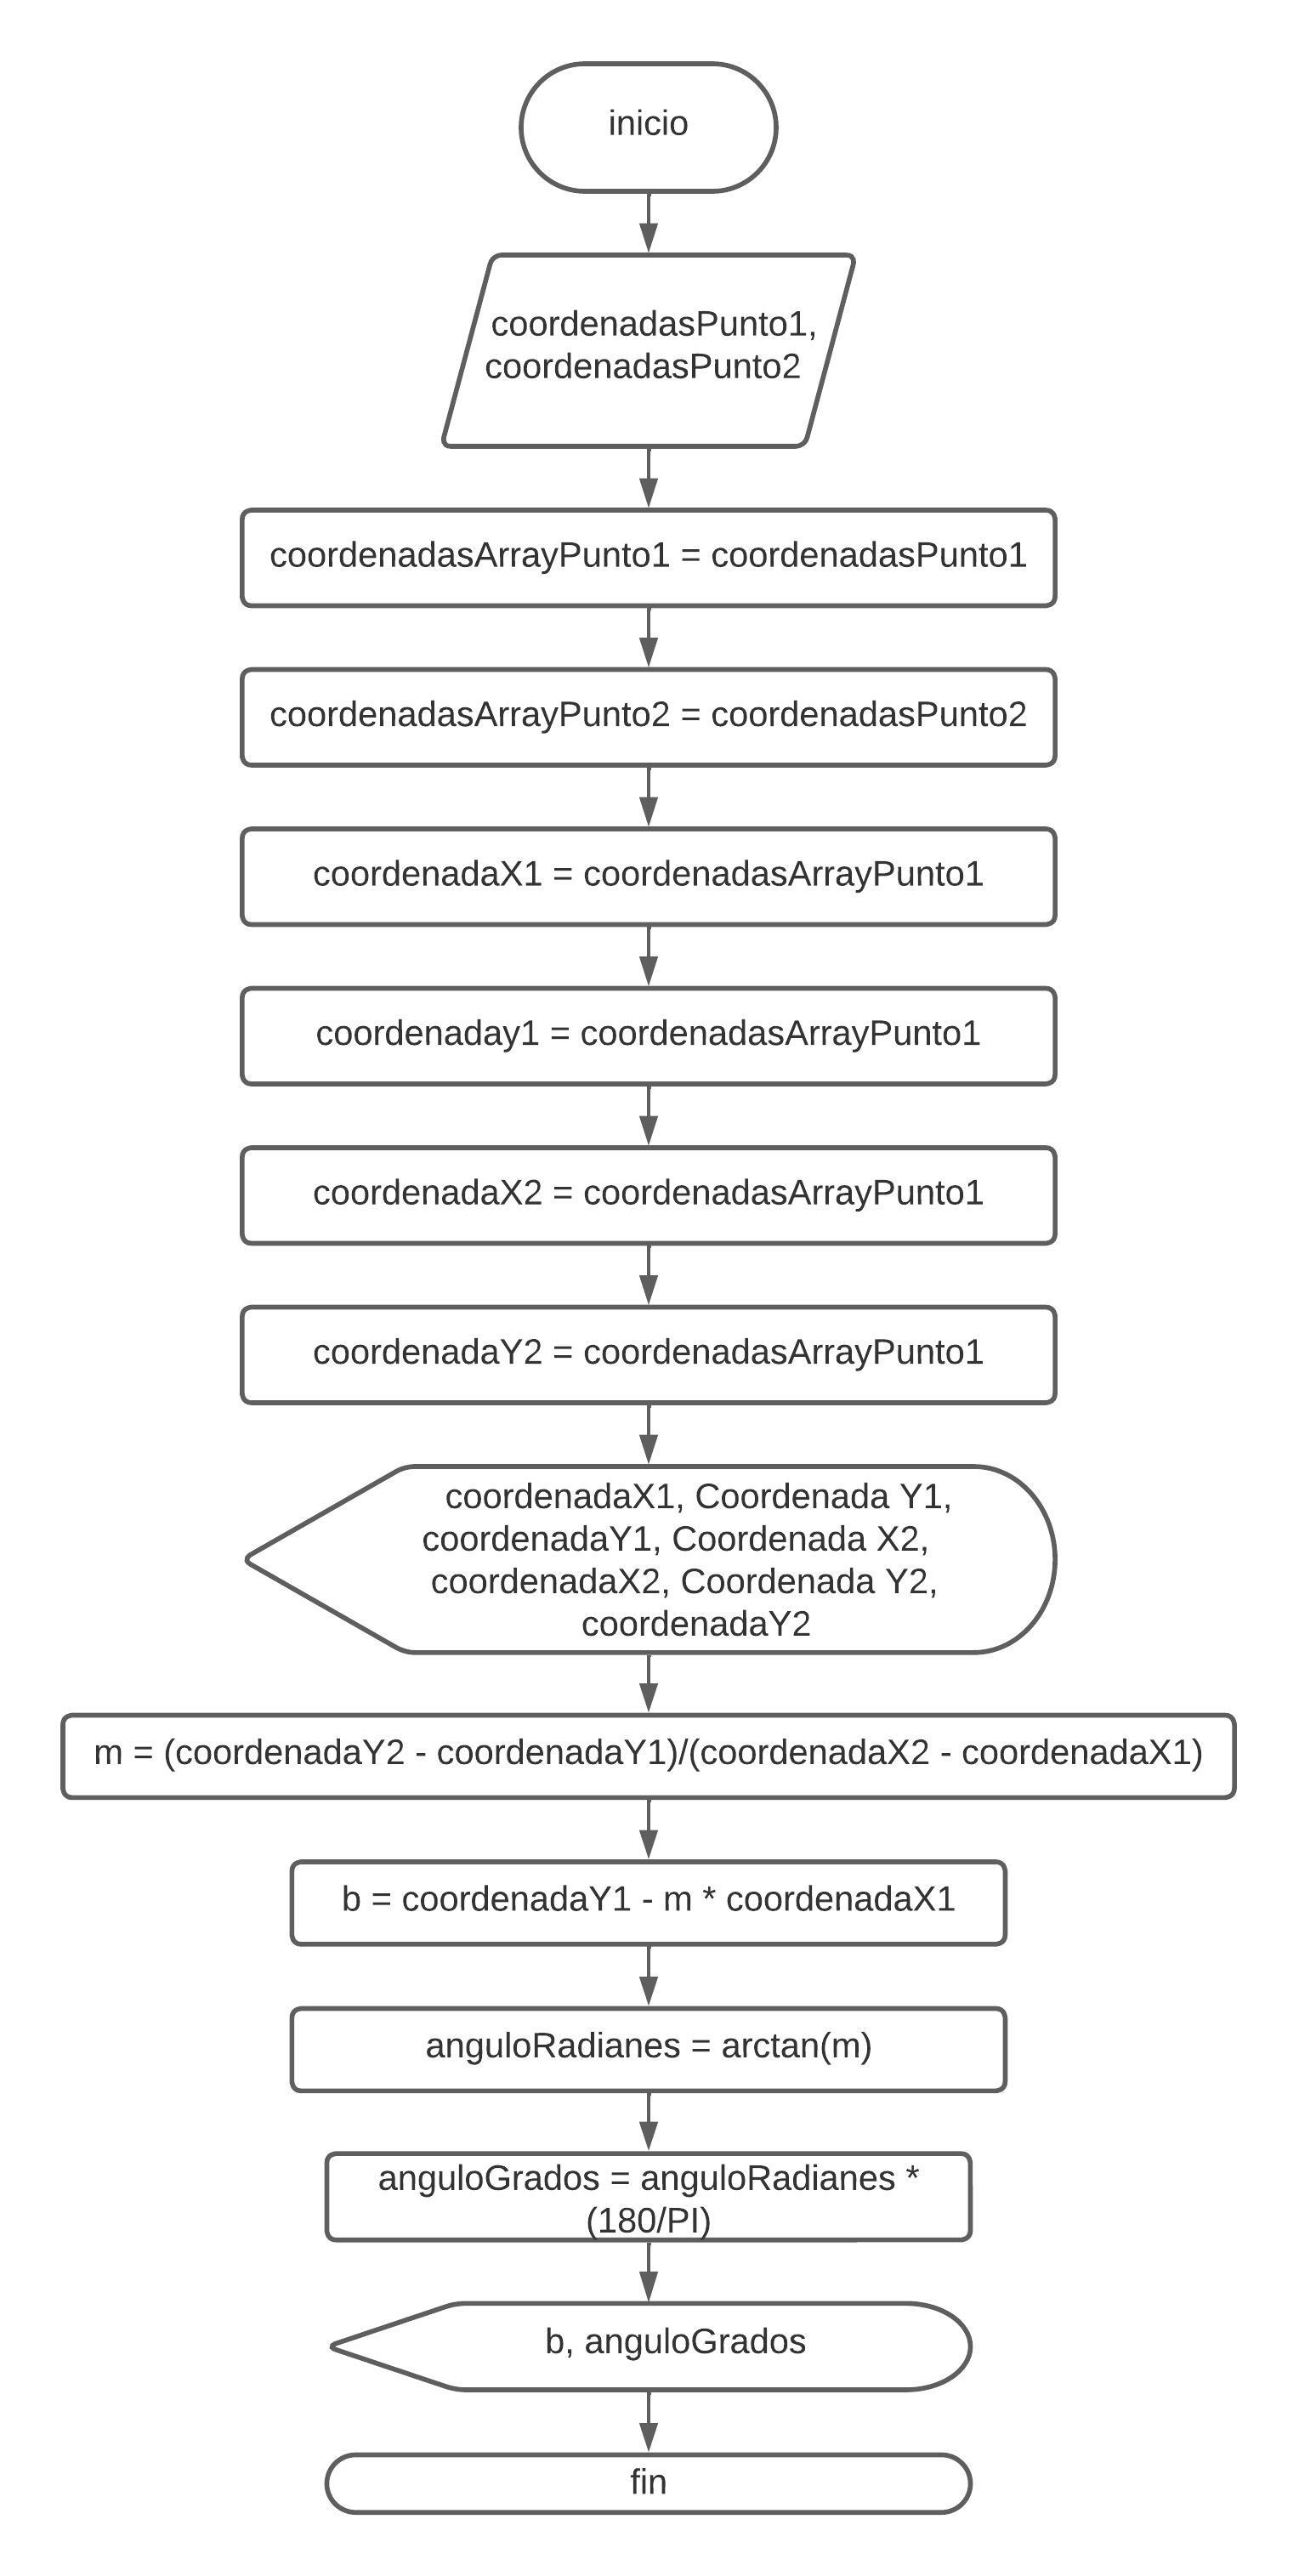
\includegraphics[width = 6cm]{Latex-imágenes/diagramaEx1.jpeg}}
\caption{Representación gráfica del algoritmo implementando la solución}
\label{fig}
\end {figure}

\subsection{Desarrollo de la solución}
Para resolver el primer problema implementamos el siguiente codigo, en el cual pide al usuario que ingrese las cordenadas el punto uno y dos separadas por una coma (,) 

\begin{javaCode}
    String coordenadasPunto1 = JOptionPane.showInputDialog("Ingrese las coordenadas del punto1(X y Y) separadas por una coma(,): ");
        
        String coordenadasPunto2 = JOptionPane.showInputDialog("Ingrese las coordenadas del punto2(X y Y) separadas por una coma(,): ");
\end{javaCode}

despues separamos los valores que el usurio ingreso, para separarlos usamos el metodo split()

\begin{javaCode}
        
        String[] coordenadasArrayPunto1 = coordenadasPunto1.split(",");
        String[] coordenadasArrayPunto2 = coordenadasPunto2.split(",");
\end{javaCode}

después con los datos ya separados los imprimimos uno por uno según los valores que ingreso el usuario, para después empezar a calcular el ángulo interno y la intersección 

\begin{javaCode}
 
        JOptionPane.showMessageDialog(null, "Coordenada X1: " + coordenadaX1 + "\n" +"Coordenada Y1: " + coordenadaY1 + "\n" + "Coordenada X2: " + coordenadaX2 + "\n" + "Coordenada Y2: " + coordenadaY2);

    double m = (coordenadaY2 - coordenadaY1)/(coordenadaX2 - coordenadaX1);
        

        double b = coordenadaY1 - m * coordenadaX1;
        
        double anguloRadianes = Math.atan(m);
        double anguloGrados = anguloRadianes * (180/Math.PI);
\end{javaCode}

y por ultimo imprimimos los resultados del ángulo interno de la recta y de la intersección 

\begin{javaCode}
     JOptionPane.showMessageDialog(null, "La intersección de la recta: " + b + "\n" + "El ángulo interno: "+anguloGrados);
\end{javaCode}

\subsection{Depuración de pruebas}

\begin{table}[h!]
  \centering
  \caption{Tabla de corridas para el Ejercicio 1.}
  \label{tab:tabla_ejemplo}
  \begin{tabular}{|c|c|c|c|c|c|}
    \hline
    \textbf{$X1$} & \textbf{$Y1$} & \textbf{$X2$} & \textbf{$Y2$} & \textbf{intersección} & \textbf{ángulo} \\
    \hline
    1 & 2 & 2 & 3 & 1 & 45\\
    2 & 4 & 6 & 8 & 2 & 0\\
    2 & 4 & 6 & 13 & 1 & 63.4349\\
    10 & 20 & 30 & 40 & 10 & 45\\
    79 & 23 & 77 & 12 & -372 & 78.6900\\
    
    \hline
  \end{tabular}
\end{table}

\section{Formula cuadrática}
%Solución del Ejercicio 2 por medio de la metodología 6D

\subsection{Descripción del problema}
 Dada una ecuación cuadrática regresar los valores de las raíces en caso de que estén sobre el conjunto de los números reales, en caso contrario indicar que la solución esta en el conjunto de los números complejos.

\begin {figure}[ht]
\centerline{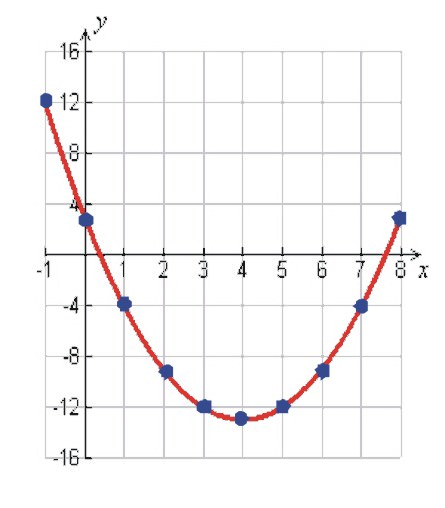
\includegraphics[width = 6cm]{Latex-imágenes/ecuacionC.jpeg}}
\caption{Gráfica de la ecuación cuadrática}
\label{fig}
\end {figure}

\subsection{Definición del problema}
Primero, tenemos que verificar que la ecuación esté en la forma estándar:

\begin{equation}
    ax^2 + bx + c = 0
\end{equation}


donde $a$, $b$ y $c$ son coeficientes reales y $x$ es la variable desconocida. Posteriormente, se deben identificar los valores de $a$, $b$ y $c$ en la ecuación. A continuación, se debe utilizar la fórmula cuadrática para encontrar las soluciones: 
\begin{equation}
x = \frac{-b \pm \sqrt{b^2 - 4ac}}{2a}
\end{equation}


Posteriormente, se sustituyen los valores de $a$, $b$ y $c$ en la fórmula cuadrática y se realizan los cálculos necesarios.\\

\subsection{Diseño de la solución}

Se realizó una representación gráfica de un algoritmo para resolver el problema
\begin {figure}[h!]
\centerline{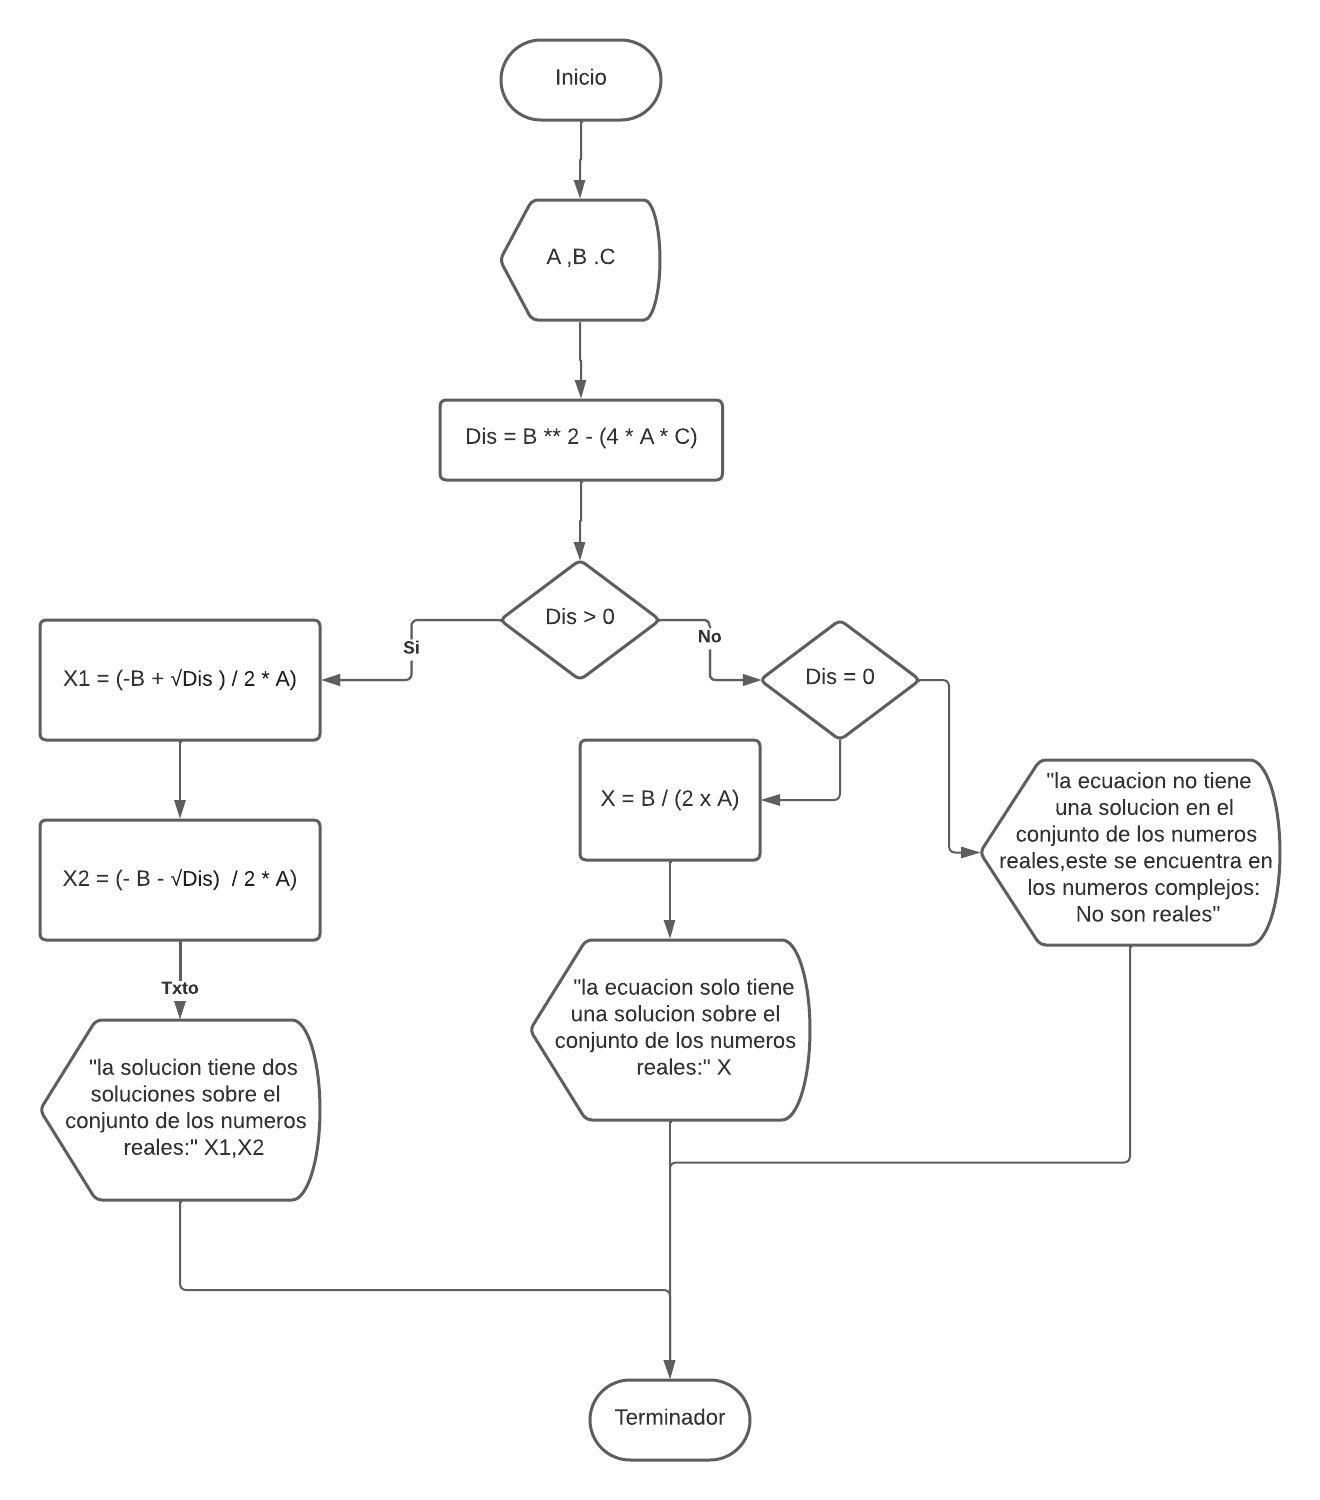
\includegraphics[width = 6cm]{Latex-imágenes/diagramaEx2.jpeg}}
\caption{Diagrama de flujo problema 2.}
\label{fig}
\end {figure}

\subsection{Desarrollo de la solución}
Para solucionar este problema tendrá que resolver los tres coeficientes de los tres parámetros de una ecuación cuadrática que se tenga, donde se desarrollara primero el discriminante y después se evaluara el mismo para determinar si hay dos soluciones, una solución o si todo es falso, no existe, para ello se implemento Este código que solicita al usuario que ingrese los coeficientes de la ecuación cuadrática $a$ $b$ $c$. 
 
\begin{javaCode}

    float a = Float.parseFloat(JOptionPane.
    showInputDialog("Ingresa coeficiente respecto al parámetro \"a\""));
        float b = Float.parseFloat(JOptionPane.
        showInputDialog("Ingresa coeficiente respecto al parámetro \"b\""));
        float c = Float.parseFloat(JOptionPane.
        showInputDialog("Ingresa coeficiente respecto al parámetro \"c\""));
        
\end{javaCode}

posterior a lo que hicimos se va a calcula el discriminante con la ecuación cuadrática.

\begin{javaCode}
  
     double discriminante = Math.pow(b, 2) - (4 * a * c);

\end{javaCode}
 

Para finalizar la discriminante pasa por la primer condición donde se obtendrán dos soluciones, la segunda solución solo nos dará una solución, en caso diferente no hay solución posible.

\begin{javaCode}
 
 if (discriminante > 0) {
            double x1 = (-b + Math.sqrt(discriminante)) / (2 * a);
            double x2 = (-b - Math.sqrt(discriminante)) / (2 * a);

            JOptionPane.showMessageDialog(null, "La solución tiene dos soluciones sobre el conjunto de los números reales:\n" +
                    "x1 = " + x1 + "\n" +
                    "x2 = " + x2);
        } else {
            if (discriminante == 0) {
                double x = -b / (2 * a);
                JOptionPane.showMessageDialog(null, "La ecuación solo tiene una solución sobre el conjunto de los números reales:\n" +
                        "x = " + x);

    
\end{javaCode}

 


\subsection{Depuración de pruebas}

\begin{table}[!ht]
\label{T:equipos}
\begin{center}
\begin{tabular}{| p{.5cm} | p{.5cm} | p{.5cm} | p{5cm} |}
\hline
\textbf{$a$} & \textbf{$b$} & \textbf{$c$} & \textbf{$x_1, x_2$ o $x$}\\
\hline
2 & 10 & 2 & -0.20, -4.79 \\
7 & 8 & 9 & "La ecuación no tiene una solución en el conjunto de los números reales, este se encuentra en los números complejos." \\
-5 & 6 & -1 & 0.2, 1.0 \\
3 & 464 & 46 & "La ecuación no tiene una solución en el conjunto de los números reales, este se encuentra en los números complejos." \\
1 & -4 & 4 & 2 \\
\hline
\end{tabular}
\caption{Tabla de corridas.}
\end{center}
\end{table}

\section{Circunferencia}
%Solución del Ejercicio 3 por medio de la metodología 6D

\subsection{Descripción del problema}
Dada una circunferencia con centro en el punto $C$ con coordenadas $(x_{1}, y_{1})$ y radio $r$, evaluar si un punto $T$ con coordenadas $(x_{2}, y_{2})$ esta dentro del área de la circunferencia.\\
\subsection{Definición de la solución}
La circunferencia es un punto que está a una misma distancia de un punto fijo llamado centro. 
La distancia de cada punto de la circunferencia al centro se llama radio.
\begin{equation}
    (x-h)^2 + (y-k)^2 =r^2
\end{equation}
\subsection{Diseño de la solución}
Para resolver estas ecuaciones y determinar si un punto T con coordenadas $(x_{2}, y_{2})$ esta dentro del área de la circunferencia con centro en el punto $C$ el cual utiliza coordenadas $(x_{1}, y_{1})$ y radio, se calcula la distancia del punto T y el centro de la circunferencia utilizando la formula de la distancia entre dos puntos $(x_{1}, y_{1})$ y $(x_{2}, y_{2})$.\\
\begin{equation}
 d = \sqrt{{(x_2 - x_1)^2 + (y_2 - y_1)^2}} 
\end{equation}
\begin {figure}[h!]
\centerline{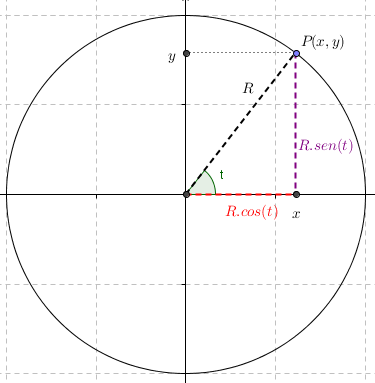
\includegraphics[width = 6cm]{Latex-imágenes/fig3.png}}
\caption{Gráfica de la ecuación.}
\label{fig}
\end {figure}
\begin{enumerate}
    \item Si $d <= r$, el punto T esta dentro del área de la circunferencia.\\
    \item Si $d > r$, el punto T esta fuera del área de la circunferencia.\\
\end{enumerate}
Se realizo un diagrama de flujo para saber como solucionar el problema.\\
\begin {figure}[h!]
\centerline{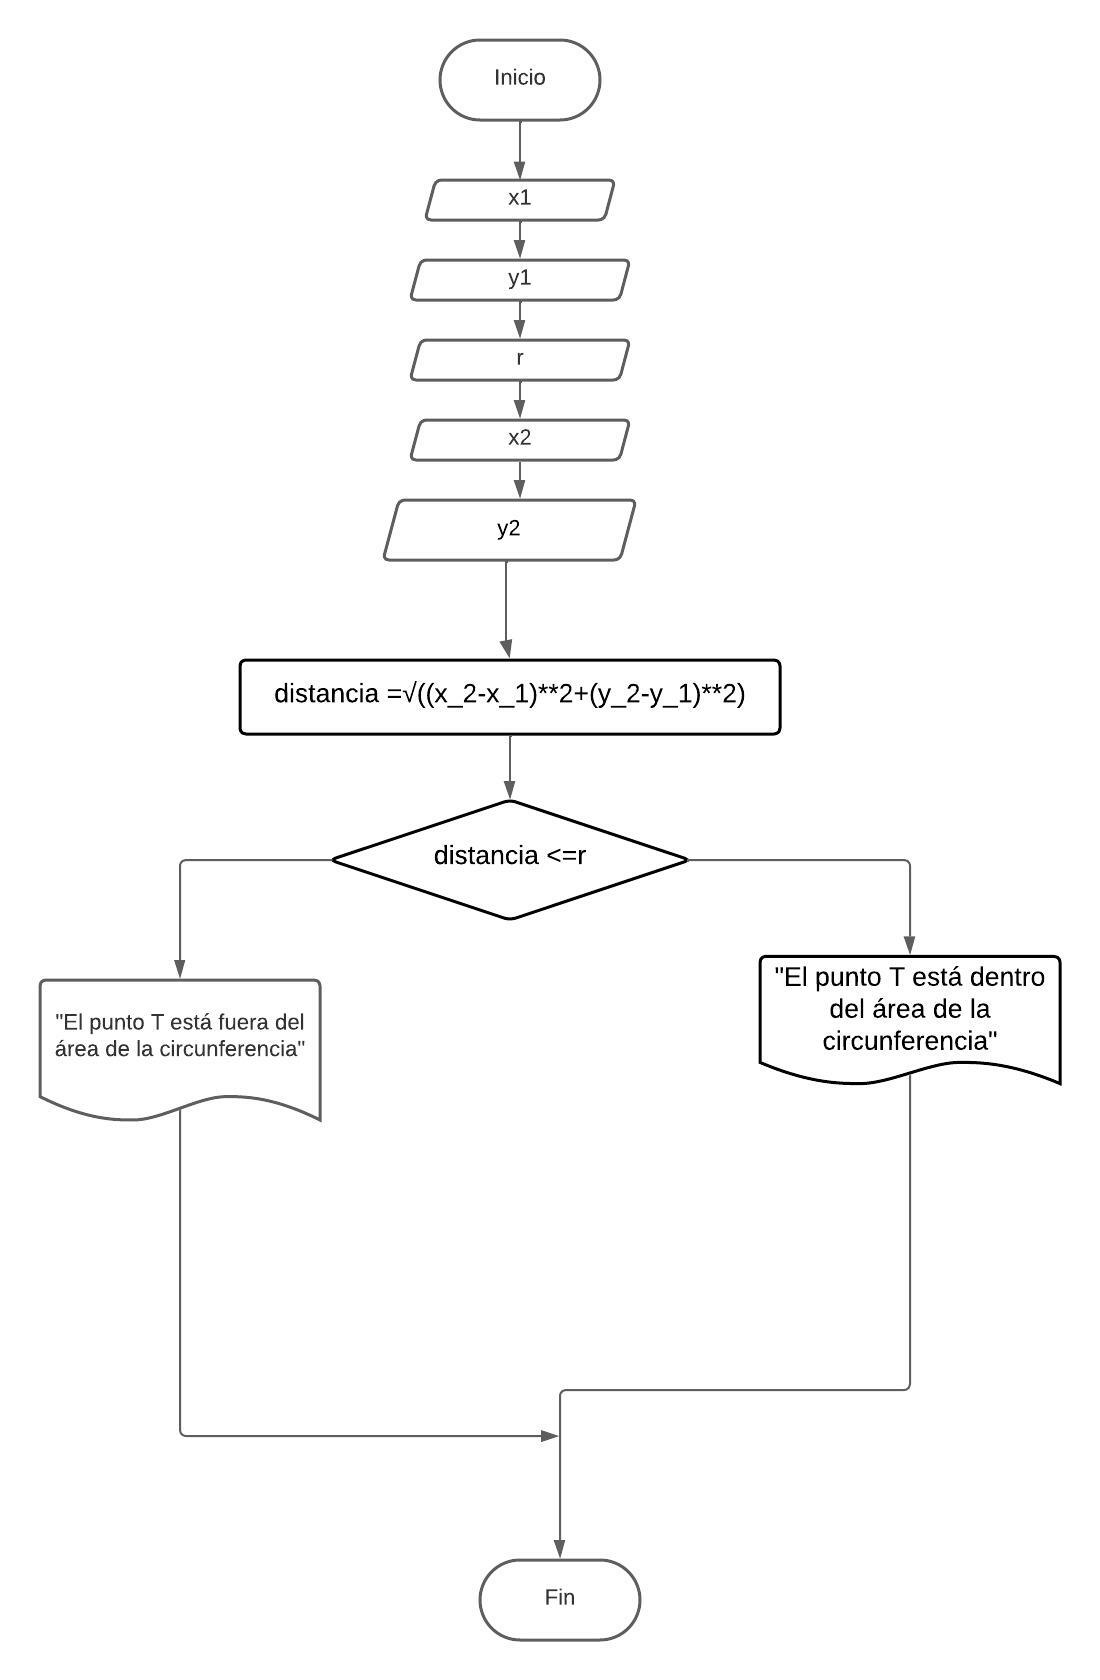
\includegraphics[width = 6cm]{Latex-imágenes/Diagrama de la circunferencia .jpeg}}
\caption{Diagrama de flujo de la solución}
\label{fig}
\end {figure}
\subsection{Desarrollo de la solución}
Para este problema se implemento este código en Apache NetBeans 14 con lenguaje en Java, donde al principio del bloque pide al usuario que ingrese las variables de la ecuación de la distancia entre dos puntos, las cuales son: $x_{1},y_{1},r,x_{2},y_{2}$
\begin{javaCode}
  double x1 = Double.parseDouble(JOptionPane.showInputDialog
       ("Ingrese la coordenada x1:"));
  double y1 = Double.parseDouble(JOptionPane.showInputDialog
       ("Ingrese la coordenada y1:"));
  double r = Double.parseDouble(JOptionPane.showInputDialog
       ("Ingrese el radio r de la circunferencia:"));
  double x2 = Double.parseDouble(JOptionPane.showInputDialog
       ("Ingrese la coordenada x2 del punto T:"));
  double y2 = Double.parseDouble(JOptionPane.showInputDialog
       ("Ingrese la coordenada y2 del punto T:"));
\end{javaCode}
Después se programo el proceso del código  el cual es la ecuación de la distancia.
\begin{javaCode}
    double distancia = Math.sqrt(Math.pow(x2 - x1, 2) + Math.pow(y2 - y1, 2));
\end{javaCode}
En el bloque final del código se presenta una condición, si la distancia es menor o igual al radio entonces el punto T está dentro del área de la circunferencia y si, no el punto T está fuera del área de la circunferencia.
\begin{javaCode}
 if (distancia <= r) {
            // Salida
            JOptionPane.showMessageDialog(null, "El punto T está dentro del área de la circunferencia.");
        } else {
            JOptionPane.showMessageDialog(null, "El punto T está fuera del área de la circunferencia.");
        }
\end{javaCode}
\subsection{Depuración y pruebas}
\begin{table}[!ht]
\label{T:equipos}
\begin{center}
\begin{tabular}{| c | c | c | c | c | c |}
\hline
\textbf{$x_{1}$} & \textbf{$y_{1}$} & \textbf{$r_x$} & \textbf{$x_{2}$} & \textbf{$y_{2}$} & \textbf{Fuera o Dentro}\\
\hline
0 & 0 & 2 & 4 & 4 & Fuera \\
0 & 1 & 2 & 3 & 4 & Fuera \\
7 & 7 & 8 & 6 & 6 & Dentro \\
20 & 10 & 9 & 5 & 5 & Fuera\\
0 & 0 & 3 & 1 & 1 & Dentro\\
\hline
\end{tabular}
\caption{Tabla de corridas.}
\end{center}
\end{table}

\section{Conversión decimal a binario}
%Solución del Ejercicio 4 por medio de la metodología 6D

\subsection{Descripción del problema}
Dado un numero decimal entero positivo o negativo regresar su equivalente en binario.

\begin {figure}[h!]
\centerline{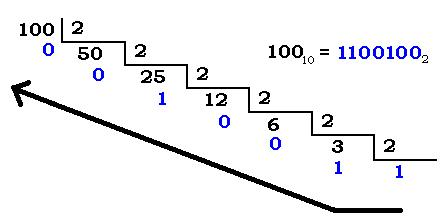
\includegraphics[width = 6cm]{Latex-imágenes/Conversion.jpeg}}
\caption{Conversión a Binario.}
\label{fig}
\end {figure}

\subsection{Definición de la solución}
Para obtener un número binario, se requiere realizar una serie de operaciones. Consiste en la división sucesiva del número decimal por dos, obteniendo el residuo en cada paso. Luego, los residuos se combinan en orden inverso para formar el número binario correspondiente. Este proceso se repite hasta que el cociente de la división sea igual a cero. Sin embargo, esta metodología presenta una problemática debido a su ineficiencia y el riesgo de cometer errores en los cálculos.

La solución planteada para abordar esta problemática ha sido la creación de una técnica computacional en el lenguaje de programación Java. Este diseño automatiza y asegura la conversión de números enteros positivos y negativos a su equivalente en el sistema binario de manera precisa y confiable. 

\subsection{Diseño de la solución}
\begin {figure}[htb]
\centerline{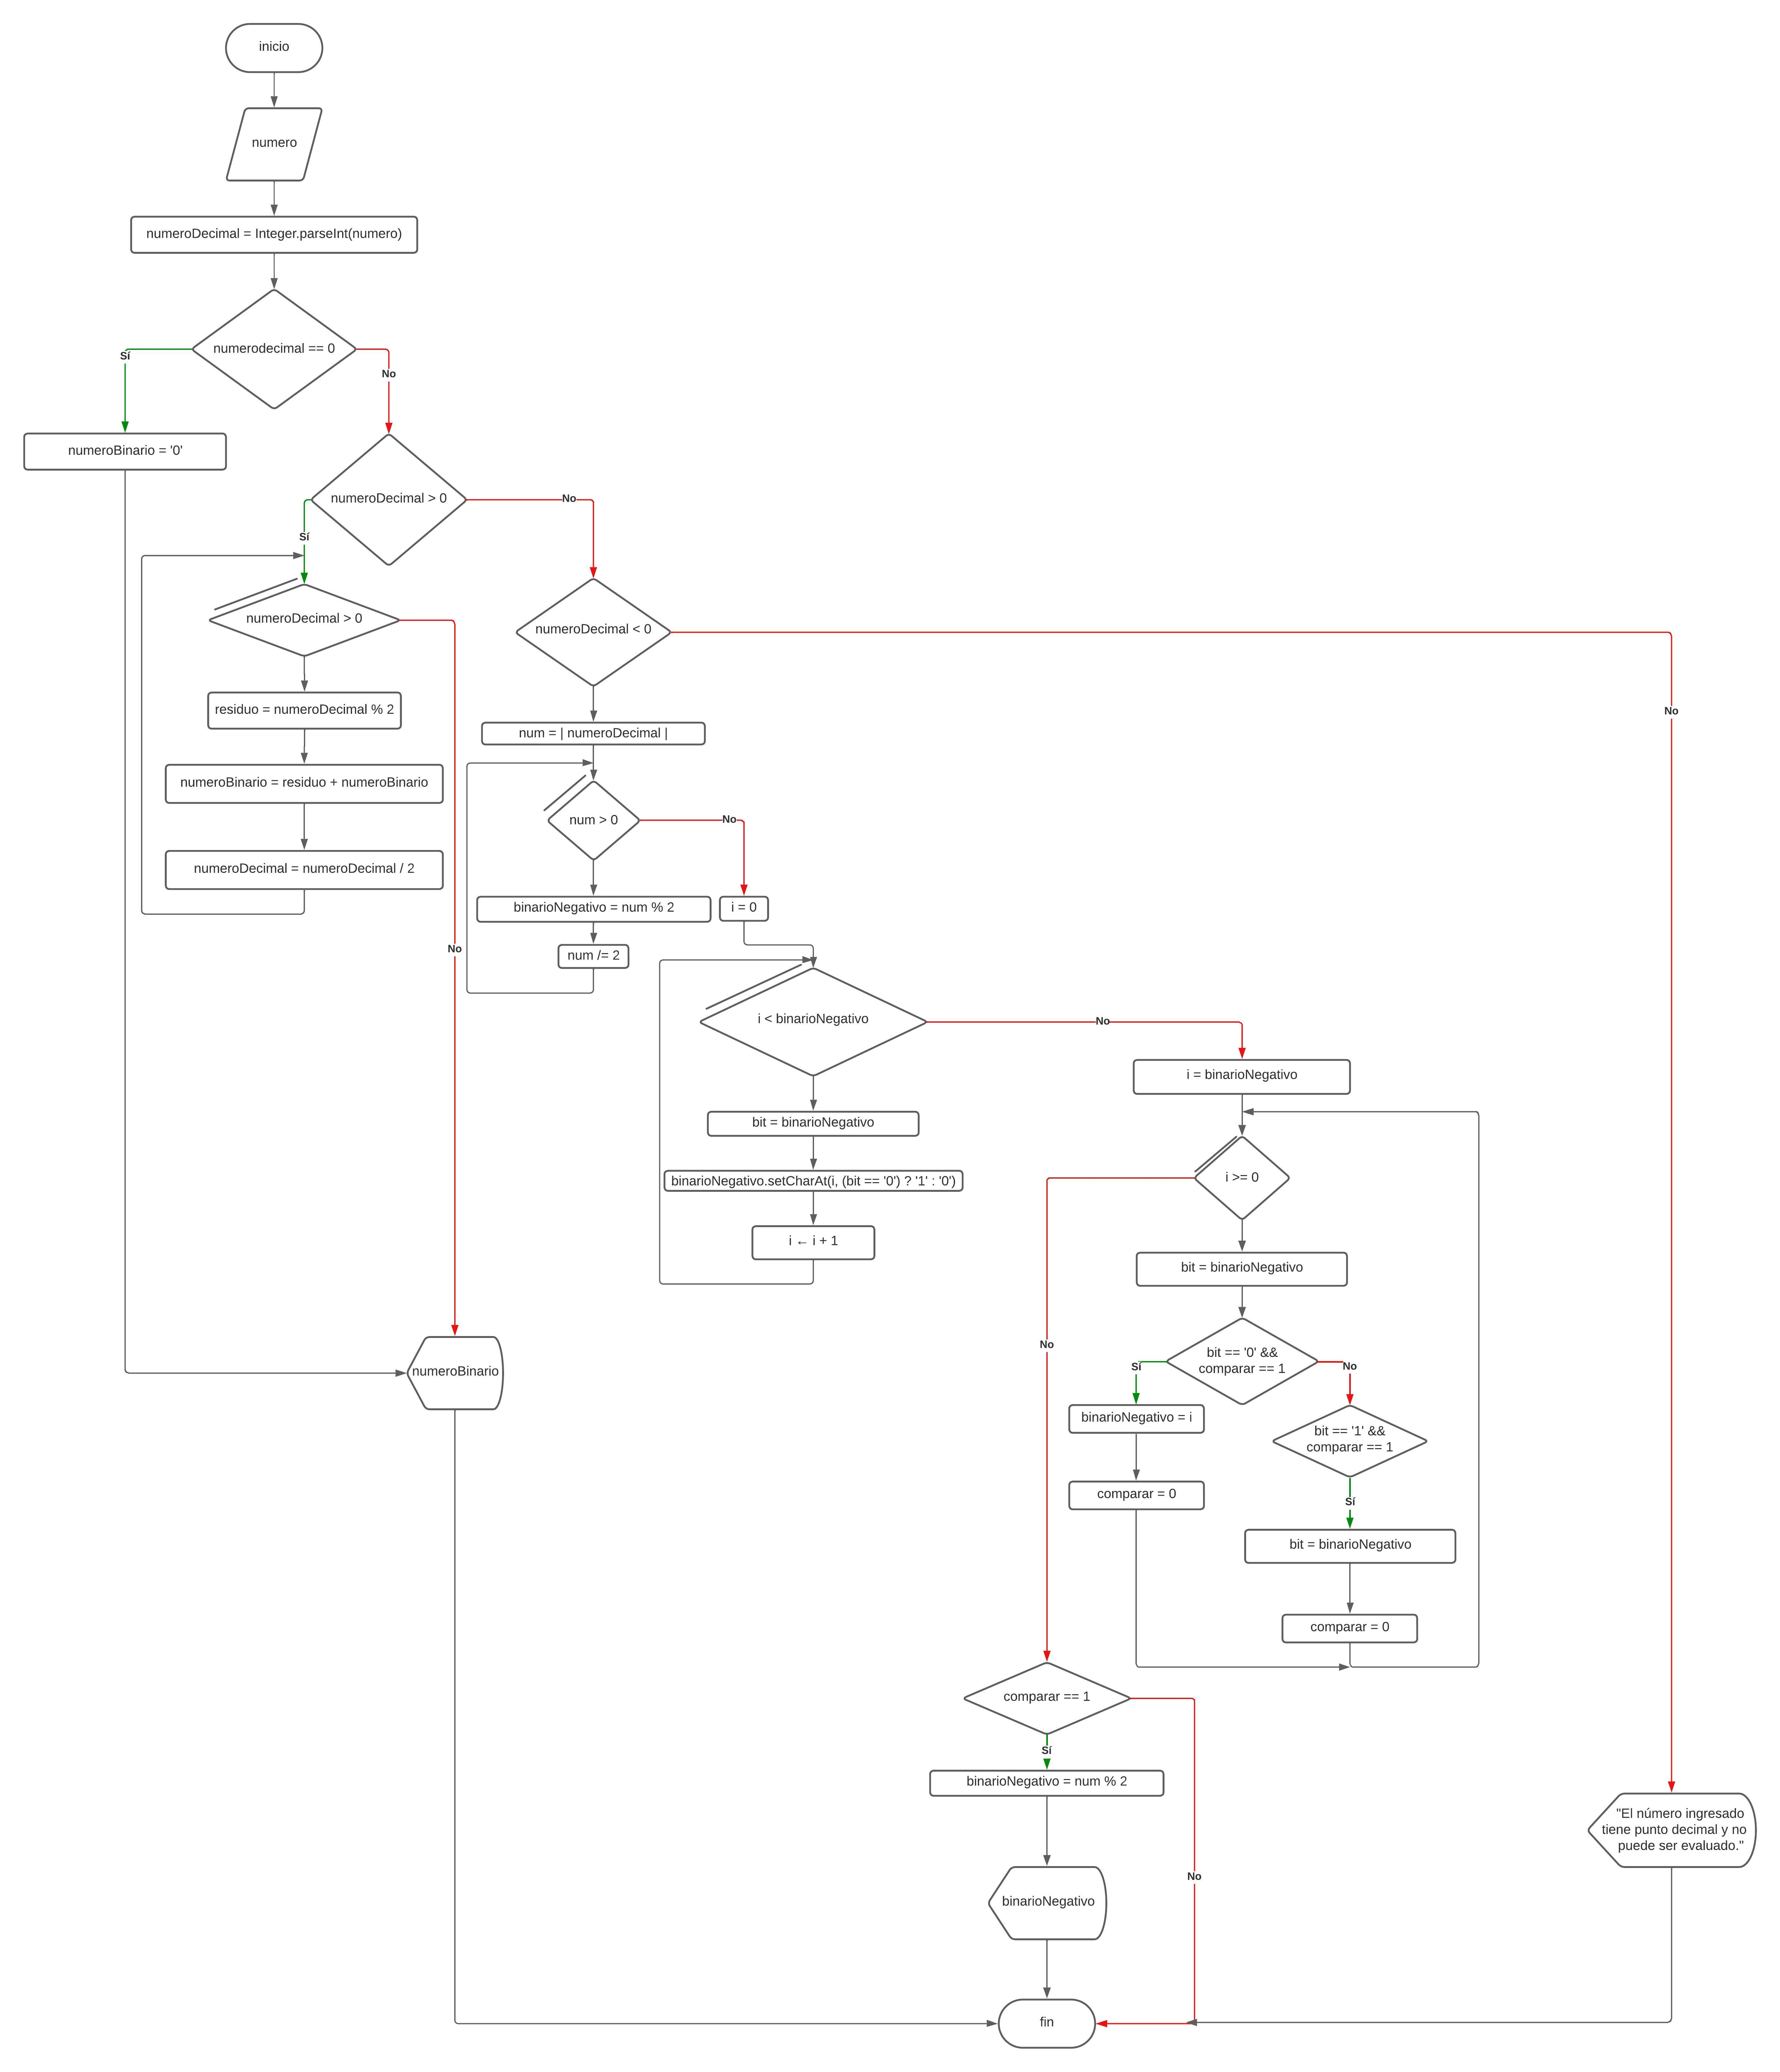
\includegraphics[width = 6cm]{Latex-imágenes/diagramaEx4.jpeg}}
\caption{Representación gráfica del algoritmo implementando la solución}
\label{fig}
\end {figure}


\subsection{Desarrollo de la solución}
En este bloque de código, se solicita al usuario que ingrese un número entero, ya sea positivo o negativo, para luego utilizarlo.
\begin{javaCode}
import javax.swing.JOptionPane;

public class decimalBinario {

    public static void main(String[] args) {
        String numero = JOptionPane.showInputDialog("Ingrese un número decimal:");
        try {
            int numeroDecimal = Integer.parseInt(numero);
            String numeroBinario = "";
\end{javaCode}
En el siguiente bloque de código se realiza una comparación con el número ingresado anteriormente. Dentro de las estructuras condicionales, se encuentra un ciclo que se encarga de descomponer el número entero en su respectiva representación binaria.
\begin{javaCode}
    if (numeroDecimal == 0) {
                numeroBinario = "0";
            } else if(numeroDecimal > 0){
                while (numeroDecimal > 0) {
                    int residuo = numeroDecimal % 2;
                    numeroBinario = residuo + numeroBinario;
                    numeroDecimal = numeroDecimal / 2;
                }
            }else 
\end{javaCode}
En este bloque de código se presenta una condición en la que, si el número entero ingresado es negativo, se realizará la conversión a su representación binaria utilizando el método del complemento A2. El complemento A2 es una operación utilizada para representar números negativos en sistemas binarios.
\begin{javaCode}
if(numeroDecimal < 0){
StringBuilder binarioNegativo = new StringBuilder();
int num = Math.abs(numeroDecimal);

while (num > 0) {
binarioNegativo.insert(0, num % 2);
num /= 2;
}
for (int i = 0; i < binarioNegativo.length(); i++) {
char bit = binarioNegativo.charAt(i);
binarioNegativo.setCharAt(i, (bit == '0') ? '1' : '0');
}

int comparar = 1;
for (int i = binarioNegativo.length() - 1; i >= 0; i--) {
char bit = binarioNegativo.charAt(i);
if (bit == '0' && comparar == 1) {
binarioNegativo.setCharAt(i, '1');
comparar = 0;
} else if (bit == '1' && comparar == 1) {
binarioNegativo.setCharAt(i, '0');
comparar = 1;
}
}
if (comparar == 1) {
binarioNegativo.insert(0, '1');
}
\end{javaCode}
Posteriormente, en otro bloque de código, se muestra en una ventana emergente la equivalencia del número entero ingresado en su respectiva representación binaria.
\begin{javaCode}
JOptionPane.showMessageDialog(null, "El número binario equivalente es: " + binarioNegativo.toString());
                return;
\end{javaCode}
De lo contrario, si se ingresó un número entero negativo, en la siguiente línea de código se mostrará una ventana emergente que contendrá el número binario negativo generado mediante su representación en complemento a 2.
\begin{javaCode}
JOptionPane.showMessageDialog(null, "El número binario equivalente es: " + numeroBinario);
\end{javaCode}
Por último, en caso de que el usuario haya ingresado un número decimal, se mostrará una ventana emergente con un mensaje.
\begin{javaCode}
JOptionPane.showMessageDialog(null, "El número ingresado tiene punto decimal y no puede ser evaluado.");
\end{javaCode}
\subsection{Depuración de pruebas}


\begin{table}[h]
  \centering
  \label{tab:tabla_ejemplo}
  \begin{tabular}{|l|c|r|}
    \hline
    \textbf{$numero$} & \textbf{numeroBinario / binarioNegativo} \\
    \hline
    -42 & 010110 \\
    -28 & 00100 \\
    5 & 101 \\
    3 & 11 \\
    10.5 & ""El número ingresado tiene  \\
     & punto decimal y no puede ser evaluado."  \\
    \hline
  \end{tabular}
  \caption{Tabla de corridas para el Ejercicio 4.}
\end{table}

\section{Conversión binario a decimal}
%solucion del problema numero 5 con las 6 D's


\subsection{Descripción del problema}
Dado un numero binario de $n$ bits regresar su equivalente en decimal.


\begin {figure}[h!]
\centerline{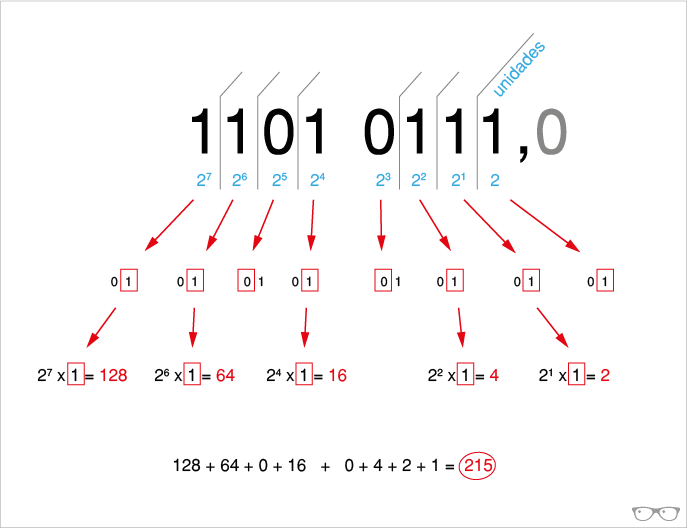
\includegraphics[width = 6cm ]{Latex-imágenes/conversion-binario-decimal.png}}
\caption{Conversión binario-decimal}
\label{fig}
\end {figure}

\subsection{Definición de la solución}
El proceso de conversión de un número binario a decimal se realiza de la siguiente manera: se enumeran los dígitos de derecha a izquierda, comenzando desde la posición cero. Se utiliza como base el número 2 y se suma el valor correspondiente a cada posición. Es decir, se eleva la base (2) al exponente de la posición en la que se encuentra el dígito, pero solo se realiza la suma si en esa posición hay un 1. Si se encuentra un 0, no se realiza ninguna suma.

\subsection{Diseño de la solución}

\begin {figure}[h!]
\centerline{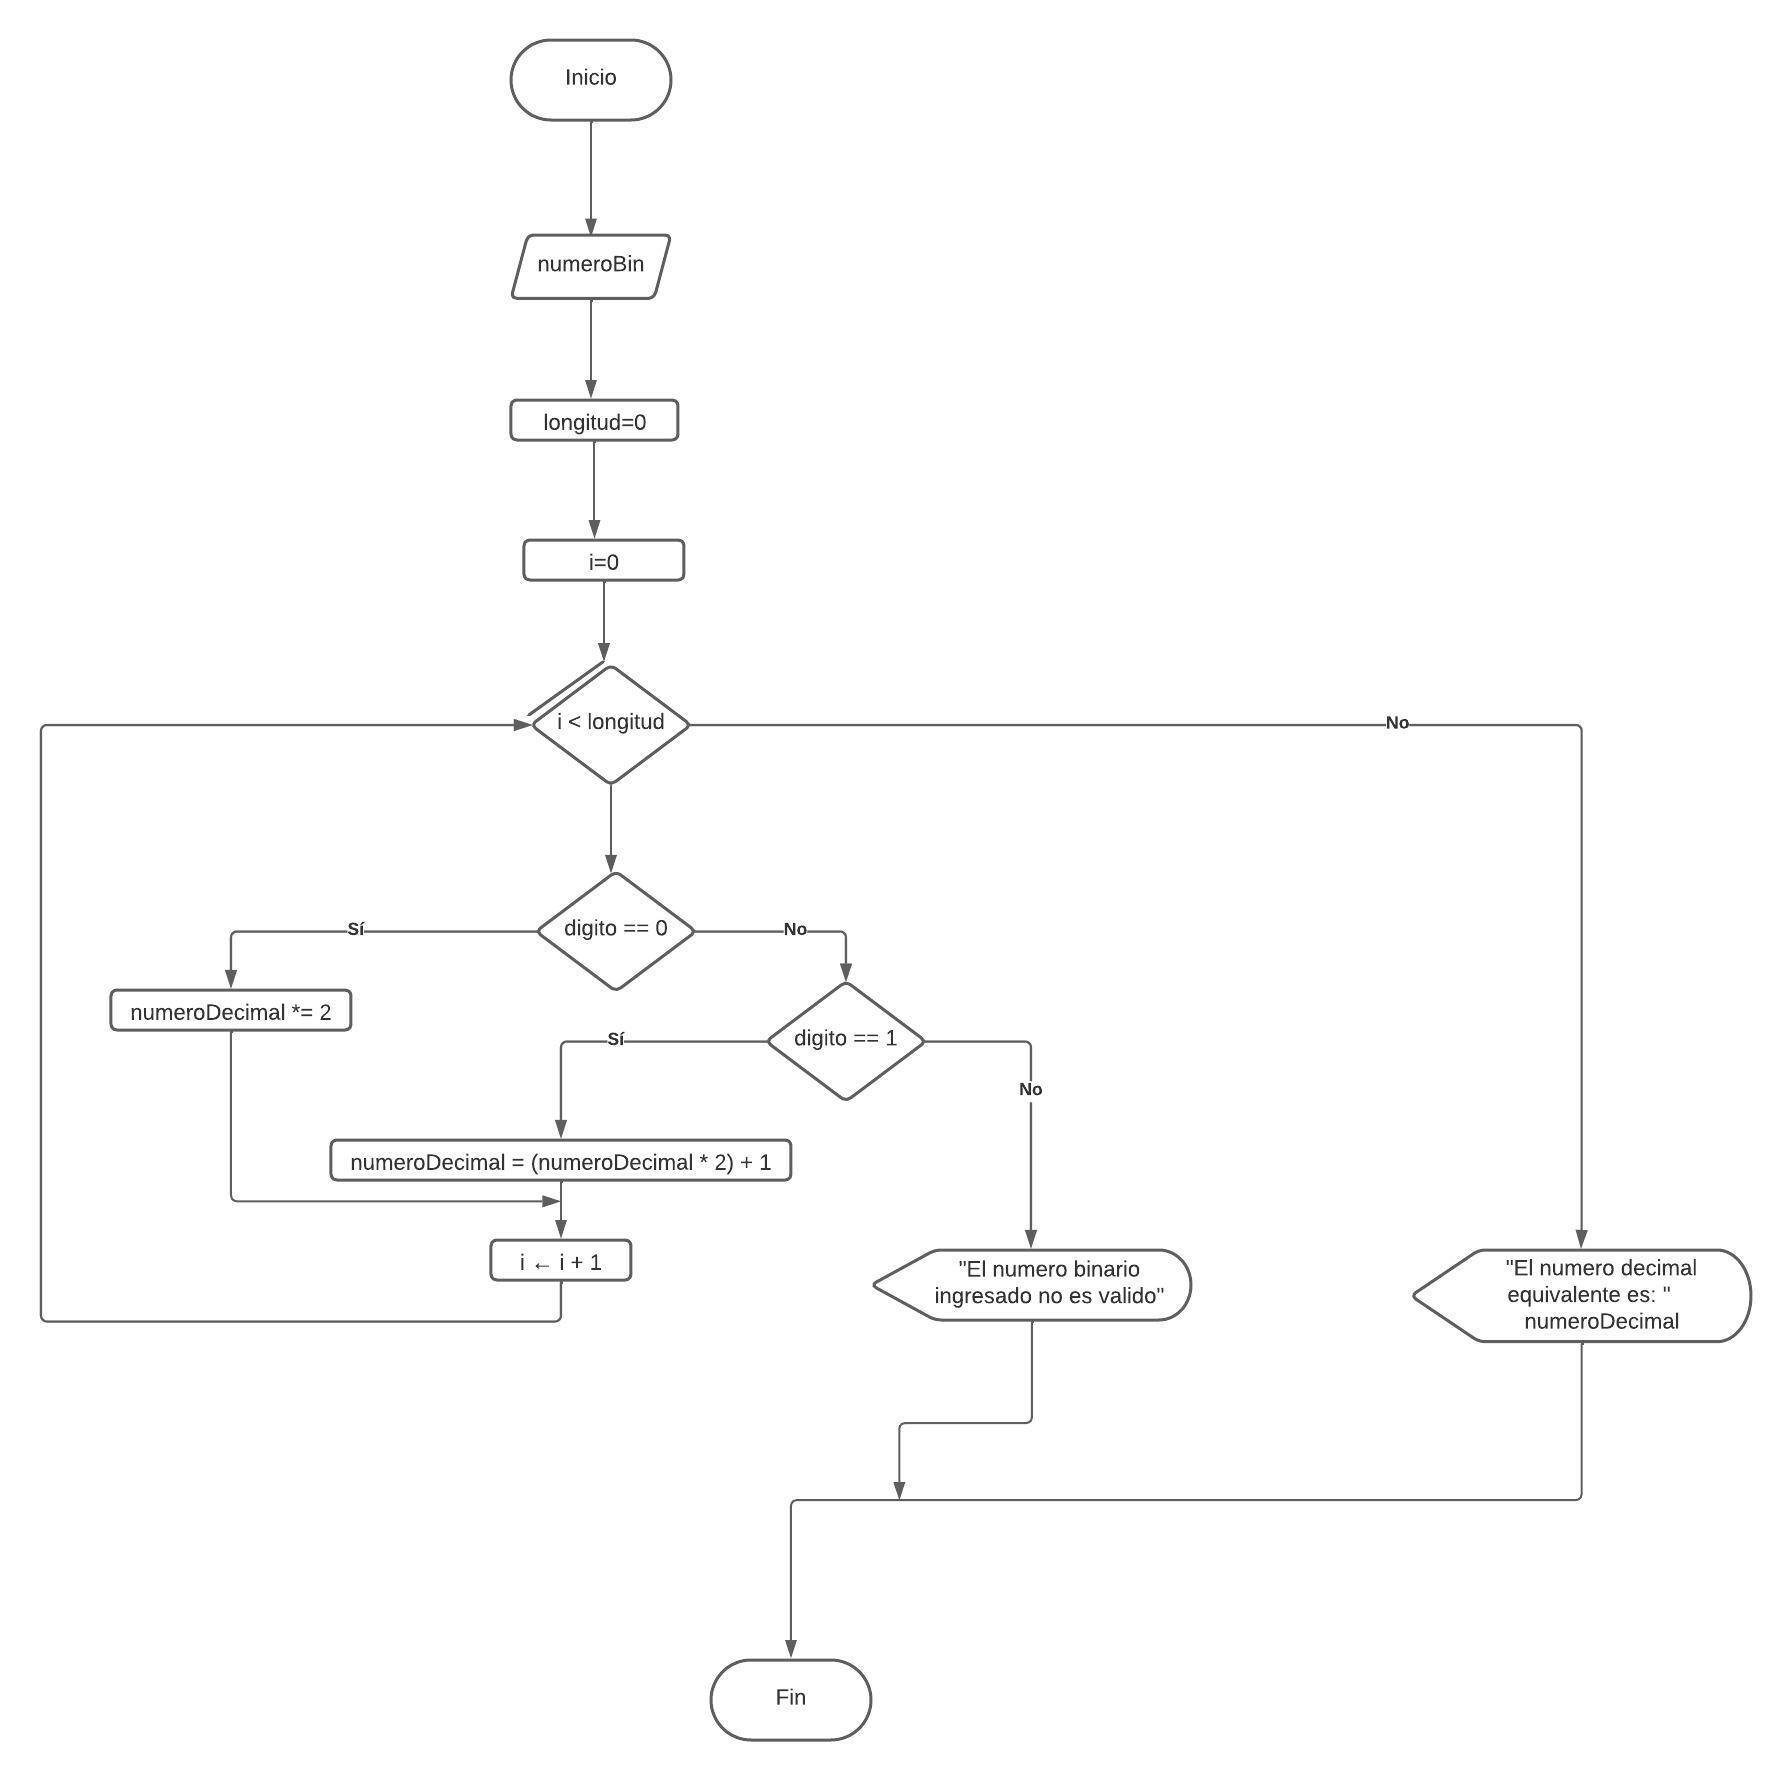
\includegraphics[width = 6cm]{Latex-imágenes/diagramaEx5.jpeg}}
\caption{Diagrama de flujo del problema 4}
\label{fig}
\end {figure}



\subsection{Desarrollo de la solución}

En el siguiente bloque de código, se muestra una ventana flotante que pide al usuario que ingrese un numero binario 

\begin{javaCode}
    String numeroBin = JOptionPane.showInputDialog("Ingresa un numero binario");
        int longitud = numeroBin.length();
        int numeroDecimal = 0;
\end{javaCode}

Después se toma ese numero y se compara si solo contiene ceros y unos, si es así el código hace las respectivas operaciones para poder obtener el numero decimal y en dado caso que el numero ingresado contenga algo mas que ceros y unos se mostrara el mensaje: " El numero binario ingresado no es valido"

\begin{javaCode}
        for (int i = 0; i < longitud; i++) {
            
            char digito = numeroBin.charAt(i);
            
            if (digito == '0') {
                numeroDecimal *= 2;
            } else if(digito == '1') {
                numeroDecimal = (numeroDecimal * 2) + 1;
            } else {
                JOptionPane.showMessageDialog(null, "El numero binario ingresado no es valido");
                return;
            }
        }
\end{javaCode}

Por ultimo si el numero ingresado solo contiene ceros y unos se muestra una ventana flotante con el resultado de la convección binario-decimal

\begin{javaCode}
JOptionPane.showMessageDialog(null, "El numero decimal equivalente es " + numeroDecimal);
\end{javaCode}

\subsection{Depuración de pruebas}

La siguiente tabla muestra el resultado de la compilación del codigo
\begin{table}[h!]
  \centering
  \caption{Tabla de corridas para el Ejercicio 5.}
  \label{tab:tabla_ejemplo}
  \begin{tabular}{|l|c|r|}
    \hline
    \textbf{$Binario$} & \textbf{Decimal} \\
    \hline
    111 & 7 \\
    10101010 & 170 \\
    675 & " El numero binario ingresado no es valido" \\
    110101 & 53 \\
    2 & " El numero binario ingresado no es valido" \\
    
    \hline
  \end{tabular}
\end{table}
\section{Tabla de verdad}
%Solucion del ejercicio por medio de la metodologia de las 6D

\subsection{Descripci\'{o}n del problema}
Dada una tabla de verdad de \textit{n} bits generar la expresión booleana que genere de manera fidedigna las salidas de esta tabla.

\subsection{Definici\'{o}n de la soluci\'{o}n}
Para llevar a cabo los teoremas booleanos, es necesario contar con datos específicos previamente obtenidos. Estos datos se obtienen a partir de una tabla de verdad que ha sido previamente creada y resuelta. Una vez que se disponen de los datos, es posible utilizar los teoremas booleanos con el fin de simplificar la expresión obtenida de la tabla de verdad, sin que esto afecte el resultado.

\subsection{Diseño de la soluci\'{o}n}

\begin {figure}[H]
\centerline{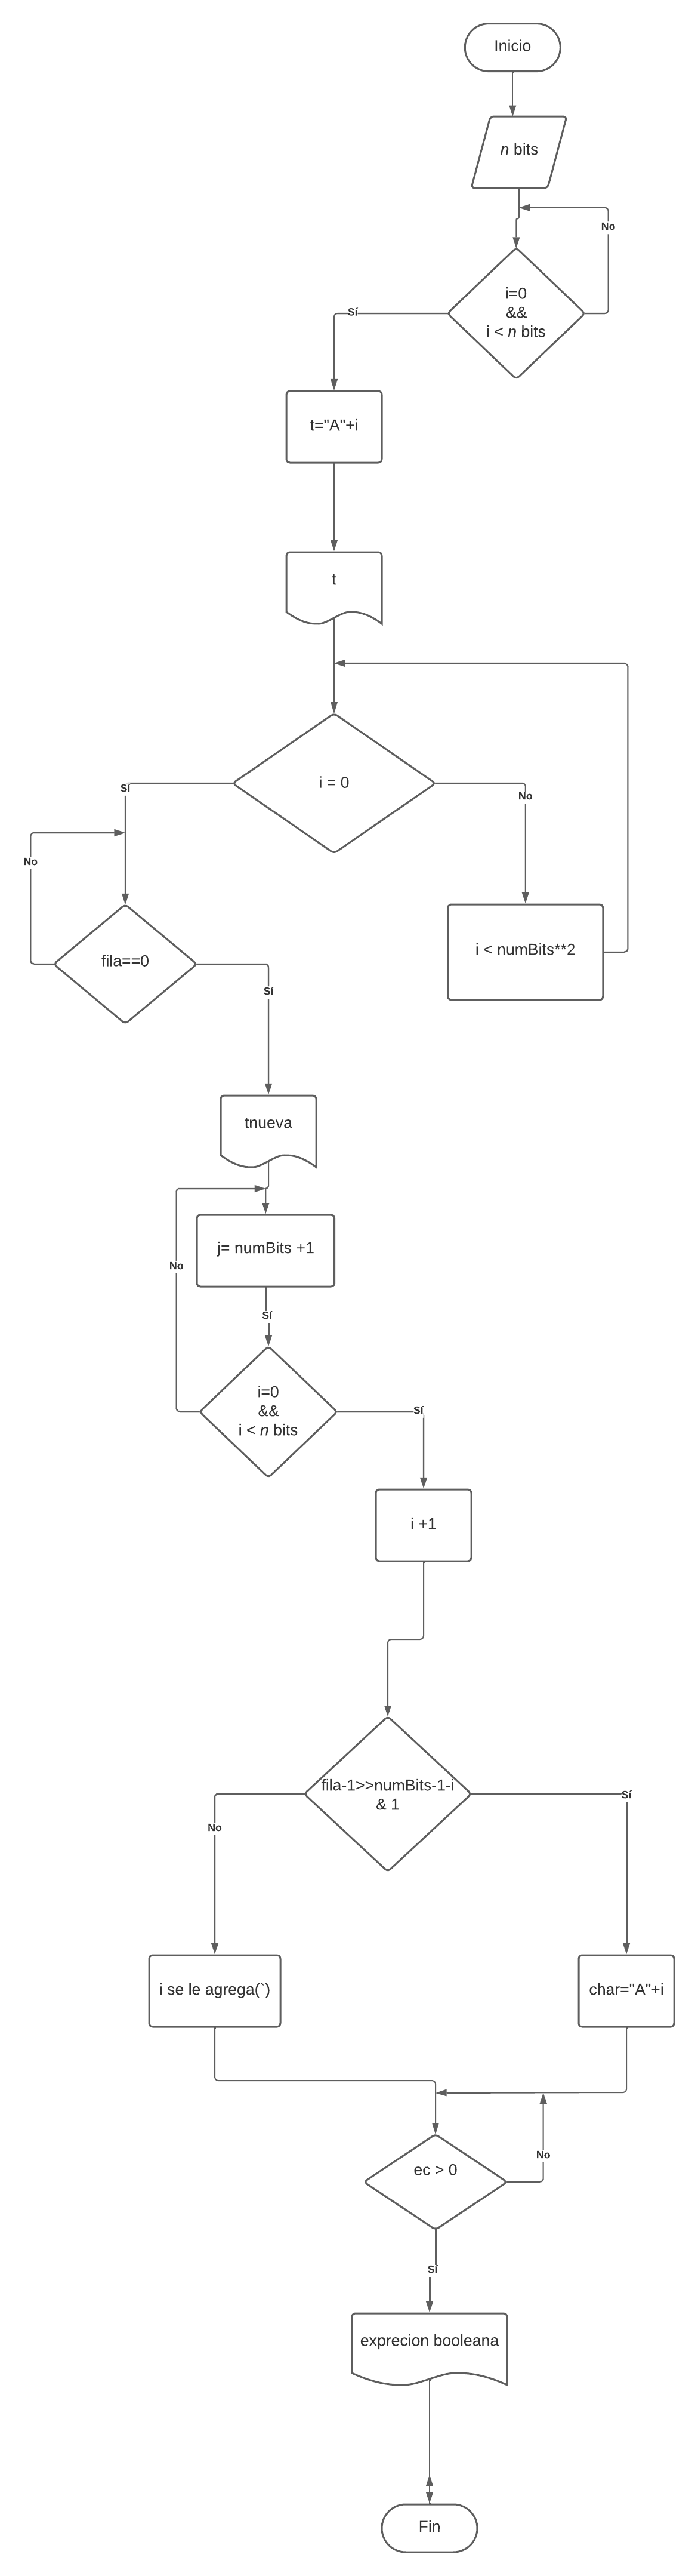
\includegraphics[width = 6cm]{Latex-imágenes/Diagrama de Tabla de Verdad (1).png}}
\caption{Diagrama de Tabla de Verdad del problema 6}
\label{fig}
\end {figure}

\subsection{Desarrollo de la soluci\'{o}n}
En el siguiente bloque de cod\'{i}go, se muestra una ventana donde pide al usuario que inserte el numero de bits.
\begin{javaCode}
     public static void main(String[] args) {
         Set<Integer> filasCambiar = new HashSet<>();
 
        String numBitsStr = JOptionPane.showInputDialog("Ingrese el Número de Bits que deberá ser la Tabla de Verdad:");
        int numBits = Integer.parseInt(numBitsStr);
\end{javaCode}

\subsection{Depuraci\'{o}n de las pruebas}
En la siguiente tabla se muestra lo antes explicado

\section{CONCLUSION}
En este documento se desarrollaron seis problemáticas de ingeniería en las cuales se realizó un exhaustivo análisis e implementación de diferentes soluciones. Estas soluciones buscan facilitar la vida de la comunidad escolar, especialmente en conceptos relacionados con la tecnología, las redes y la electrónica. El objetivo principal es brindar un gran apoyo mediante soluciones prácticas y acciones concretas que tengan un impacto positivo en aspectos clave. Además, se enfoca en abordar desafíos importantes y promover un enfoque innovador centrado en el desarrollo integral de los estudiantes.

Posteriormente, se propone brindar oportunidades de desarrollo profesional que les permitan adquirir conocimientos en temas relevantes y adaptarse a las necesidades del usuario para lograr resultados más eficientes. Esto significa que a medida que el usuario utiliza el sistema, este se vuelve cada vez más preciso. Esta orientación nos ha enseñado la importancia de la creatividad, la cooperación y la implementación práctica de los conocimientos para poder entregar un trabajo bien elaborado.
\vspace*{-8pt}


\section{AGRADECIMIENTOS}
Queremos expresar nuestro agradecimiento a la Ing.Citlali Azucena Martinez Calva tutora de nuestro grupo por el conocimiento brindado en programación y por la paciencia dada a los alumnos que desconocían sobre el tema, también al Mtro.José Martín Oropeza Méndez el cual brindo de su tiempo y transmitió sus conocimientos sobre matemáticas discretas,igual agradecemos al Doc.Francisco Javier Cuadros Romero por compartir sus experiencias y conocimientos sobre las Tics lo cual fue fundamental para obtener datos significativos y valiosos para este proyectos, agradecemos al Ing.Giovany Humberto Neri Peréz por el gran apoyo que dio al darnos accesorias para este proyecto, por la paciencia, tiempo y comprensión así como enseñarnos mas sobre calculo diferencial, también agradecemos al Lic. Agustín Soto Arista por contribuir a este proyecto, su orientación en fundamentos de investigación lo cual ayudo a redactar este proyecto y se agradece al Lic. Juan Cornejo Hernández Jefe de División de Ingeniería en TIC´s por el apoyo, sus valiosos comentarios a lo largo del semestre, la ayuda y disposición que tuvo para nosotros.
A todos ustedes, nuestros mas sinceros agradecimientos, sin su apoyo este proyecto no habría sido posible.


\def\refname{Referencias}

\begin{thebibliography}{1}

\bibitem{AA1}
 Khan Academy, October 20, 2023, Tangent lines and rates of change,
  https://www.khanacademy.org/math/calculus-all-old/taking-derivatives-calc/using-the-formal-definition-of-derivative-calc/a/tangent-lines-and-rates-of-change

\bibitem{BB1}
  Fórmula de la distancia (video). (n.d.). Khan Academy. https://es.khanacademy.org/math/geometry/hs-geo-analytic-geometry/hs-geo-distance-and-midpoints/v/distance-formula

\bibitem{CC1}
Comprender la fórmula de la cuadrática (artículo) | KhanAcademy.
  (s. f.). Khan Academy.https://es.khanacademy.org/math/algebra-home/alg-quadratics/alg-solving-quadratics-using-the-quadratic-formula/a/quadratic-formula-explained-article

\bibitem{DD1}
  Villalpando, Francisco, and Andrés García Sandoval. Matemáticas Discretas. Grupo Editorial Patria, 21 Oct. 2014.
  
\bibitem{EE1}
   “Números Binarios (Artículo).” Khan Academy, es.khanacademy.org/computing/ap-computer-science-principles/x2d2f703b37b450a3:digital-information/x2d2f703b37b450a3:binary-numbers/a/bits-and-binary.

\bibitem{FF1}
    Villalpando, Francisco, and Andrés García Sandoval. Matemáticas Discretas. Grupo Editorial Patria, 21 Oct. 2014.
\end{thebibliography}\vspace*{-8pt}

\begin{IEEEbiography}{Jacob Salas Andrea}{\,} es una estudiante de la ingeniería en Tecnologías de la Información y las Comunicaciones en el Instituto Tecnológico Superior del Occidente del Estado de Hidalgo, criada en el Mezquital, municipio de Santiago de Anaya, Hidalgo, a lo largo de su vida ha tenido diversos intereses, como la danza, el baloncesto, la musica,  pero el mas grande es por la tecnología, ya que le sorprende lo mucho que avanza en corto tiempo. El objetivo de Andrea es completar sus estudios universitarios en ITICs, con especialización en redes, sueña con trabajar en el extranjero ejerciendo su carrera. \\
\href{https://github.com/AndyJacobSalas}{Github de Andrea}
\end{IEEEbiography}

\begin{IEEEbiography}{Calva Abraham}{\,} es un estudiante de la ingeniería en Tecnologías de la información y Comunicaciones del Instituto Tecnológico Superior del Occidente del Estado de Hidalgo nacido en Rodhe Islan EEUU. Y criado en Mixquiahuala Hidalgo, que a lo largo del tiempo a tenido una gran pasión por el fútbol, los videojuegos y la tecnología.\\
\href{https://github.com/AbrahamCalva}{Github de Abraham}
%\vadjust{\vfill\pagebreak}
\end{IEEEbiography}

\begin{IEEEbiography}{Martinez Escamilla Erick}{\,} es un estudiante de la ingeniería en Tecnologías de la Información y las Comunicaciones del Instituto Tecnológico Superior del Occidente del Estado de Hidalgo, que a lo largo del tiempo a tenido una gran pasión por el fútbol, los videojuegos, el espacio y la tecnología.\\
\href{https://github.com/ErickEsca}{Github de Erick}
\end{IEEEbiography}

\begin{IEEEbiography}{Vidal Ceron Jean Paul}{\,} Jean Paul Vidal Cerón es un estudiante de Ingeniería en Tecnologías de la Información y Comunicaciones del Instituto Tecnológico Superior del Occidente del Estado de Hidalgo. Tiene una gran pasión por los videojuegos, tanto nuevos como retro, el anime y, sobre todo, por la programación. Nació en Actopan, Hidalgo, y creció en Mixquiahuala de Juárez, Hidalgo. A lo largo del tiempo, ha desarrollado una curiosidad e interés por la informática y los avances innovadores en tecnología.
El objetivo principal de Jean Paul es completar sus estudios universitarios en ingeniería de TIC con especialización en IoT. Su mayor satisfacción al estar en esta especialidad es poder crear nueva tecnología eficiente para la comunidad y contribuir en la ayuda a la sociedad.\\
\href{https://github.com/JeanPaulVidal}{Github de Jean Paul}
\end{IEEEbiography}

\begin{IEEEbiography}{Barrera Rojo Roberto}{\,} es un estudiante de la ingeniería en Tecnologías de la Información y Comunicaciones con una pasión por el fútbol, MMA y por los videojuegos y criado en Mixquiahuala de Juárez Hidalgo, desde temprana edad demostró un gran interés por las artes marciales mixtas y las consolas de videojuegos. Roberto se encanta por el taekwondo y videojuegos. Estos medios le han enseñado la importancia de la perseverancia y el trabajo en equipo. El objetivo principal de Roberto es completar sus estudios universitarios en ITICs y jugar en la selección de fútbol de esa misma universidad. Sueña con trabajar en el campo de full stack, encargándose de coordinar todas las acciones entre el front-end y del back-end ya sea de una web o una app\\
\href{https://github.com/RobertoBarreraa}{Github de Roberto}
\end{IEEEbiography}

\end{document}

